\documentclass[a4paper]{article}
\usepackage{latexsym}
\usepackage[a4paper]{geometry}
\usepackage{color}
\usepackage{listings}
\usepackage[pdftex]{graphicx}
\usepackage{subfig}

\definecolor{Blue}{rgb}{0,0,0.5}
\definecolor{Green}{rgb}{0,0.75,0.0}
\definecolor{LightGray}{rgb}{0.6,0.6,0.6}
\definecolor{DarkGray}{rgb}{0.3,0.3,0.3}
\lstset{language=Matlab,
   keywords={function,uint8,uint16,uint32,double,break,case,catch,continue,else,elseif,end,for,global,if,otherwise,persistent,return,switch,try,while},
   basicstyle=\ttfamily\small,
   breaklines=true,
   keywordstyle=\bfseries\color{Blue},
   commentstyle=\itshape\color{LightGray},
   stringstyle=\color{Green},
   numbers=left,
   numberstyle=\tiny\color{DarkGray},
   stepnumber=1,
   numbersep=10pt,
   backgroundcolor=\color{white},
   tabsize=2,
   showspaces=false,
   showstringspaces=false,
   captionpos=b}

%Boldface text for type writer font
\usepackage{bold-extra} %\DeclareFontShape{OT1}{cmtt}{bx}{n}{<5><6><7><8><9><10><10.95><12><14.4><17.28><20.74><24.88>cmttb10}{}

%Break words properly at the end of a line (which isn't sloppy...)
\sloppy

%Use command \exercise for each exercise
\newcounter{exerciseCount}
\setcounter{exerciseCount}{0}
\newcommand{\exercise}[1]{\addtocounter{exerciseCount}{1} \noindent \medskip {\large \textsf{\textbf{Exercise \arabic{exerciseCount} \--- #1}}} \par}
\renewcommand{\theenumi}{\textsf{\textbf{\alph{enumi}}}}

%Use command \code for code snippets
\newcommand{\code}[1]{\textnormal{\texttt{#1}}}



\title{\textsf{Image Processing \\ lab 1}}
\author{Klaas Kliffen \and Jan Kramer}
\date{\today}

\begin{document}
\maketitle

\exercise{Zooming and shrinking by pixel replication}

\exercise{Histogram equalization}

\exercise{Spatial filtering}
\begin{enumerate}
\item
\lstinputlisting{../lab1ex3/IPfilter.m}

\item
\lstinputlisting{../lab1ex3/IPSobel.m}

\begin{center}
\begin{figure}
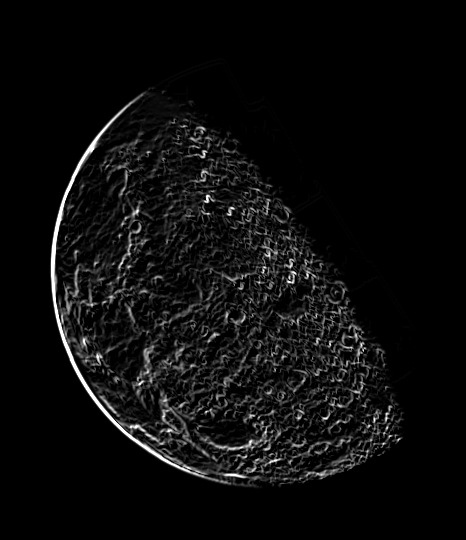
\includegraphics[width=\textwidth]{../lab1ex3/blurrymoonsobel.png}
\caption{The result of the application of the IPSobel function to blurrymoon.tif}
\end{figure}
\end{center}

\end{enumerate}

\section{Task distribution}

%table?

\end{document}
